\chapter{FPGA NES kártya ismertetése}

A NES hardverének újragondolásából \aref{fig:PCB-blockdiagram} ábrán látható blokk diagramot készítettem, ez a nyomtatott huzalozott kártyák tervezésének első lépése. Már itt érdemes feltüntetni a különböző áramköri elemek közti kommunikációs utakat (busz típusokat), illetve ezek irányát. Ez alapján a diagram alapján, pedig elkezdődhet a különböző komponensek keresése, ezt követően át kell gondolnunk ezek fogyasztását és feszültség szintjeit ezekből az adatokból pedig megtervezhető a kártya táp ellátása is (a mi esetünkben már kiegészítettem ezzel a blokk diagramot). 

\begin{figure}[H]
	\centering
	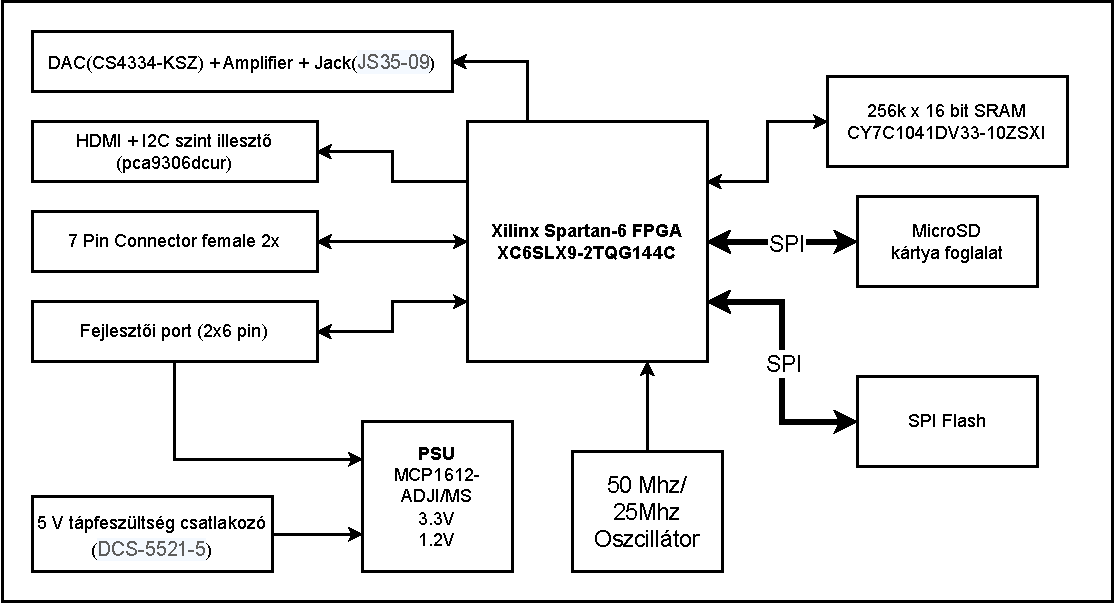
\includegraphics[width=150mm, keepaspectratio]{figures/NES-board-blockdiagram}
	\caption{NES kártya blokkdiagramja}
	\label{fig:PCB-blockdiagram}
\end{figure}

A komponensek, közül az FPGA chip kiválasztása a legnehezebb, ennek menete általában az, hogy megpróbáljuk felmérni a hardverünk méretét és ez alapján választunk megfelelő méretű chip-et. A mi esetünkben az egyik legkomplexebb elem a 6502-es 8-bites processzor amely méretét az OpenCores weboldalon található nyílt forráskódú hardver tervek alapján megbecsülhetjük körülbelül 1000 LUT-ra. Mivel NES hardver működéséhez három fő komponens kell (CPU, APU, PPU) ezek méretét egyesével felülbecsülhetjük a legkomplexebb alkatrész méretével, így összesen 3000 LUT-ot kapunk. Ehhez még érdemes a VGA jel elő állítását (HDMI jel kódolása), illetve az audió jel kezelését még hozzá számolni, erre is jó felső becslés az 1000 LUT. Végül még érdemes tartalékkal is számolni ezért egy 5000-6000 LUT-al rendelkező FPGA chip valószínűleg elég nagy ahhoz, hogy a teljes projekt elférjen benne. Fontos kritérium még, hogy DCM-el illetve PLL-el rendelkezzen a chip az egyedi órajelek előállítása érdekében (például a 250 MHz a VGA bit-ek kiadásához), ezen kívül még Blokk-RAM-ra is szükség lesz legalább akkorára mint a NES hardverének belső memóriája (például Név táblák 2 kilobájt).  

%todo kell e ide a konzulens hivatkozása Szerencsére a konzulensem jóvoltából, szert tettem
A feladat megvalósításához egy Spartan-6-os Xilinx FPGA állt a rendelkezésemre, amely megfelel a fent említett összes elvárásnak. Ez a chip nagyban meggyorsította a nyáktervezés menetét is, mivel az egyetemi Spartan-6-os fejlesztő kártyák fő komponense is ez az FPGA volt (erről itt olvashatunk részletesebben \cite{spatan6}). Ezt a fejlesztő kártyát vettem alapul a NES kártyám fejlesztő portjának kialakítása, az SPI flash bekötése, illetve a táp vonalak kialakítása során is. 
	
A kártyán az alábbi komponensek találhatók:

\begin{itemize}
	\item \emph{FPGA:} Xilinx XC6SLX9-2TQG144C típusú Spartan-6-os FPGA, amely lehetővé teszi összetettebb logikák és
	mikroprocesszoros rendszerek megvalósítását. Az eszköz főbb jellemzői:
		\begin{itemize}
			\item 5720 darab 6 bemenetű LUT és 11440 darab flip-flop
			\item 32 darab 18 kilobites blokk-RAM
			\item 16 darab DSP48A1 blokk (elő összeadó, 18 x 18 bites előjeles szorzó és akkumulátor)
			\item 4 darab DCM (Digital Clock Manager) és 2 darab PLL (Phase Locked Loop) modul
		\end{itemize} 
	\item \emph{Memóriák a program és az adatok tárolására:}
		\begin{itemize}
			\item Egy 256k x 16 bites (512 kB), 10 ns-os aszinkron SRAM (Cypress CY7C1041DV33-10ZSXI)
			\item Egy 32 Megabites SPI buszos soros FLASH memória (Atmel AT25DF321A), amely
			konfigurációs memóriaként is szolgál az FPGA számára
		\end{itemize}
	\item \emph{Egy MicroSD memóriakártya foglalat:}
		\begin{itemize}
			\item Teljes MicroSD kártya protokoll
			\item Egyszerű SPI protokoll
		\end{itemize}
	\item \emph{Beviteli eszközök:}
		\begin{itemize}
			\item Két eredeti 7 lábas NES (GamePAD) kontroller csatlakozók
			\item Reset és PROG gombok
		\end{itemize}	
	\item \emph{Képfeldolgozás:}
		\begin{itemize}
			\item HDMI csatlakozó 
			\item I2C szint illesztő (PCA9306DCUR típusú), a HDMI audió vonalainak illesztéséhez 
		\end{itemize}
	\item \emph{Audio:}
		\begin{itemize}
			\item Digitális-analóg átalakító (DAC), CS4334-KSZ típusú  
			\item 100mW Erősítő TS486IST típus (fülhallgatókhoz)
			\item CUI SJ1-3553NG 3.5mm Jack csatlakozó
		\end{itemize}
	\item \emph{Tápegységek:} MCP1612-ADJI/MS típusú szinkron Buck konverterek
	\item \emph{Egy 50 MHz-es oszcillátor} 
	\item \emph{Csatlakozó a LOGSYS fejlesztői kábel számára} 
\end{itemize}
	
\section{Tápellátás}
	
	A tápellátás kialakítása a Logsys Spartan-6-os fejlesztői kártyáéhoz hasonló \cite{spatan6}. A NES kártya 5 V-os tápfeszültségről működik. Ezt a tápellátást, vagy a fejlesztő kábelről kapja az eszköz, vagy egy külső 5 V-os forrásból. A külső egyenfeszültségű forrás Shottky diódával védtem, illetve a kártyát töltést jelző zöld led-del is elláttam (PWR). 
	
	Az 5 V-os forrást két azonos típusú step down (Buck) konverterrel 3.3 V-ra és 1.2 V-ra konvertálom. Alapvetően az FPGA működéséhez kell a két feszültség szint. A 3.3 V az I/O vonalakért, DCM, PLL, és konfigurációért felelős, az 1.2 V pedig az FPGA belső magjának kell. Ezt a két tápvonalat az FPGA dokumentációja alapján (a táp lábaihoz közel) elláttam a megfelelő mennyiségű csatoló (coupling) és hidegítő (bulk) kapacitásokkal a stabil működés végett. A 3.3 V-ot a kártyán található többi alkatrész is használja (SRAM, MicroSDkártya, kontrollerek, a fejlesztő kábel is megkapja mint JTAG referencia feszültség ként stb.). Illetve a kártya a HDMI csatlakozó, DAC és erősítő komponensek esetén, a tápellátás 5 V-ját is felhasználja. A tápellátás schematik rajzát \aref{sec:PSU} függelékben láthatjuk. 
	 
\section{Órajel források}
	
	A NES kártyán a Logsys fejlesztő kártyához hasonlóan, egy 50 MHz-es oszcillátort helyeztem el. Az FPGA, vagy a fejlesztő portról érkező CLK-től kapja az órajelét, vagy ezt az 50 MHz-es CLK-t használja. Ahhoz, hogy az FPGA használhassa ezeket az órajeleket egy-egy órajel bemeneti lábára (GCLK) kellet ezeket bekötni. Az oszcillátor segéd áramkörét \aref{sec:OSC-JTAG} függelékben láthatjuk. % és órajel források bekötését pedig \aref{tab:FPGA-OSCpin} táblázatban olvashatjuk.
	
%	\begin{table}[H]
%		\footnotesize
%		\centering
%		\begin{tabular}{|l|l|}
%			\hline
%			\rowcolor[HTML]{C0C0C0} 
%			\multicolumn{1}{|c|}{\cellcolor[HTML]{C0C0C0}{\color[HTML]{333333} \textbf{Órajel forrás}}} & \multicolumn{1}{c|}{\cellcolor[HTML]{C0C0C0}{\color[HTML]{333333} \textbf{FPGA láb}}} \\ \hline
%			50 MHz-es oszcillátor                                                                       & P85                                                                                   \\ \hline
%			Fejlesztői port CLK vonala                                                                  & P95                                                                                   \\ \hline
%		\end{tabular}
%		\caption{FPGA órajel forrásainak bekötése}
%		\label{tab:FPGA-OSCpin}
%	\end{table}
	
\section{Memória - SRAM}
	
	A választott asszinkron SRAM mérete 256 k x 16 bit (byte-okban mérve 512 k), ez a méret megfelel \aref{sec:Game-store} fejezetben tárgyalt játék méreteknek (csak egy NES játék nem fog beleférni ebbe a RAM-ba). A választott memória előnye, hogy 10 ns elérési idejű asszinkron, statikus RAM, egyszerű kezeléssel. Ez azért jelent előnyt a konzol hardveres emulálása szempontjából, mert nem fogja ennek működését befolyásolni a memória elérési idő (a későbbiekben az elérést igazíthatjuk az általunk választott időzítéshez). DRAM esetén sokkal több időzítési paraméterrel kell számolni ez természetesen jóval megnehezíti a időzítés kritikus hardver létrehozását.
	
	Az SRAM 18 bites címmel rendelkezik, amellyel megcímezhetők a 2 byte-osával az adataink (256 k cím). A RAM-ból kiolvasott, illetve beírandó adatokat pedig a 16 bit-es adat vonalak olvasásával és írásával érhetjük el. Az SRAM vezérlésétől függően kiolvasható vagy írható egyszerre mind a 16 bit, de van byte-os elérési mód is.
	
	Az SRAM szabványos vezérlési felülettel rendelkezik. Tehát következő vezérlő jelek segítségével tudjuk irányítani (ezek mindegyike negált logikájú): chip engedélyezés CSn, írás engedélyezése WEn, olvasás engedélyezés OEn, alsó byte engedélyezés LBn, végül pedig a felső byte engedélyezés UBn. A memória olvasási és írási idő diagramjait \acite{sram} adatlapon olvashatjuk, kiegészítő áramkörét pedig \aref{sec:SRAM-SPI-Flash} függelékben láthatjuk.     
	
%	\begin{table}[H]
%		\footnotesize
%		\centering
%		\begin{tabular}{|lccccccccc|}
%			\hline
%			\rowcolor[HTML]{C0C0C0} 
%			\multicolumn{10}{|l|}{\cellcolor[HTML]{C0C0C0}\textbf{Címbusz}}                                                                                                                                                                                                                                                                                                                                                                                                                                                                                                                                                                                                                                      \\ \hline
%			\rowcolor[HTML]{EFEFEF} 
%			\multicolumn{1}{|l|}{\cellcolor[HTML]{EFEFEF}SRAM}                            & \multicolumn{1}{c|}{\cellcolor[HTML]{EFEFEF}A0}                         & \multicolumn{1}{c|}{\cellcolor[HTML]{EFEFEF}A1}                         & \multicolumn{1}{c|}{\cellcolor[HTML]{EFEFEF}A2}                         & \multicolumn{1}{c|}{\cellcolor[HTML]{EFEFEF}A3}                         & \multicolumn{1}{c|}{\cellcolor[HTML]{EFEFEF}A4}                         & \multicolumn{1}{c|}{\cellcolor[HTML]{EFEFEF}A5}                         & \multicolumn{1}{c|}{\cellcolor[HTML]{EFEFEF}A6}                         & \multicolumn{1}{c|}{\cellcolor[HTML]{EFEFEF}A7}                         & A8   \\ \hline
%			\rowcolor[HTML]{EFEFEF} 
%			\multicolumn{1}{|l|}{\cellcolor[HTML]{EFEFEF}{\color[HTML]{333333} FPGA láb}} & \multicolumn{1}{c|}{\cellcolor[HTML]{EFEFEF}{\color[HTML]{333333} P47}} & \multicolumn{1}{c|}{\cellcolor[HTML]{EFEFEF}{\color[HTML]{333333} P46}} & \multicolumn{1}{c|}{\cellcolor[HTML]{EFEFEF}{\color[HTML]{333333} P45}} & \multicolumn{1}{c|}{\cellcolor[HTML]{EFEFEF}{\color[HTML]{333333} P44}} & \multicolumn{1}{c|}{\cellcolor[HTML]{EFEFEF}{\color[HTML]{333333} P43}} & \multicolumn{1}{c|}{\cellcolor[HTML]{EFEFEF}{\color[HTML]{333333} P34}} & \multicolumn{1}{c|}{\cellcolor[HTML]{EFEFEF}{\color[HTML]{333333} P33}} & \multicolumn{1}{c|}{\cellcolor[HTML]{EFEFEF}{\color[HTML]{333333} P32}} & P30  \\ \hline
%			\multicolumn{1}{|l|}{SRAM}                                                    & \multicolumn{1}{c|}{A9}                                                 & \multicolumn{1}{c|}{A10}                                                & \multicolumn{1}{c|}{A11}                                                & \multicolumn{1}{c|}{A12}                                                & \multicolumn{1}{c|}{A13}                                                & \multicolumn{1}{c|}{A14}                                                & \multicolumn{1}{c|}{A15}                                                & \multicolumn{1}{c|}{A16}                                                & A17  \\ \hline
%			\multicolumn{1}{|l|}{FPGA láb}                                                & \multicolumn{1}{c|}{P29}                                                & \multicolumn{1}{c|}{P7}                                                 & \multicolumn{1}{c|}{P6}                                                 & \multicolumn{1}{c|}{P5}                                                 & \multicolumn{1}{c|}{P2}                                                 & \multicolumn{1}{c|}{P1}                                                 & \multicolumn{1}{c|}{P139}                                               & \multicolumn{1}{c|}{P138}                                               & P137 \\ \hline
%		\end{tabular}
%		\caption{SRAM memória címbusz bekötése}
%		\label{tab:FPGA-MEM-SRAMpin}
%	\end{table}
%		
%	\begin{table}[H]
%		\footnotesize
%		\centering
%		\begin{tabular}{|lcccccccc|}
%			\hline
%			\rowcolor[HTML]{C0C0C0} 
%			\multicolumn{9}{|l|}{\cellcolor[HTML]{C0C0C0}\textbf{Adatbusz}}                                                                                                                                                                                                                                                                                                                                                                                                                                                                                                                                                                                  \\ \hline
%			\rowcolor[HTML]{EFEFEF} 
%			\multicolumn{1}{|l|}{\cellcolor[HTML]{EFEFEF}SRAM}                            & \multicolumn{1}{c|}{\cellcolor[HTML]{EFEFEF}D0}                         & \multicolumn{1}{c|}{\cellcolor[HTML]{EFEFEF}D1}                         & \multicolumn{1}{c|}{\cellcolor[HTML]{EFEFEF}D2}                         & \multicolumn{1}{c|}{\cellcolor[HTML]{EFEFEF}D3}                         & \multicolumn{1}{c|}{\cellcolor[HTML]{EFEFEF}D4}                         & \multicolumn{1}{c|}{\cellcolor[HTML]{EFEFEF}D5}                         & \multicolumn{1}{c|}{\cellcolor[HTML]{EFEFEF}D6}                         & D7                         \\ \hline
%			\rowcolor[HTML]{EFEFEF} 
%			\multicolumn{1}{|l|}{\cellcolor[HTML]{EFEFEF}{\color[HTML]{333333} FPGA láb}} & \multicolumn{1}{c|}{\cellcolor[HTML]{EFEFEF}{\color[HTML]{333333} P40}} & \multicolumn{1}{c|}{\cellcolor[HTML]{EFEFEF}{\color[HTML]{333333} P17}} & \multicolumn{1}{c|}{\cellcolor[HTML]{EFEFEF}{\color[HTML]{333333} P21}} & \multicolumn{1}{c|}{\cellcolor[HTML]{EFEFEF}{\color[HTML]{333333} P22}} & \multicolumn{1}{c|}{\cellcolor[HTML]{EFEFEF}{\color[HTML]{333333} P23}} & \multicolumn{1}{c|}{\cellcolor[HTML]{EFEFEF}{\color[HTML]{333333} P24}} & \multicolumn{1}{c|}{\cellcolor[HTML]{EFEFEF}{\color[HTML]{333333} P26}} & {\color[HTML]{333333} P27} \\ \hline
%			\multicolumn{1}{|l|}{SRAM}                                                    & \multicolumn{1}{c|}{D8}                                                 & \multicolumn{1}{c|}{D9}                                                 & \multicolumn{1}{c|}{D10}                                                & \multicolumn{1}{c|}{D11}                                                & \multicolumn{1}{c|}{D12}                                                & \multicolumn{1}{c|}{D13}                                                & \multicolumn{1}{c|}{D14}                                                & D15                        \\ \hline
%			\multicolumn{1}{|l|}{FPGA láb}                                                & \multicolumn{1}{c|}{P8}                                                 & \multicolumn{1}{c|}{P9}                                                 & \multicolumn{1}{c|}{P10}                                                & \multicolumn{1}{c|}{P11}                                                & \multicolumn{1}{c|}{P12}                                                & \multicolumn{1}{c|}{P14}                                                & \multicolumn{1}{c|}{P15}                                                & P16                        \\ \hline
%		\end{tabular}
%		\caption{SRAM memória adatbusz bekötése}
%		\label{tab:FPGA-DATA-SRAMpin}
%	\end{table}
%
%	\begin{table}[H]
%		\footnotesize
%		\centering
%		\begin{tabular}{|llllcc|}
%			\hline
%			\multicolumn{6}{|l|}{\cellcolor[HTML]{C0C0C0}\textbf{Vezérlő jelek}}                                                                                \\ \hline
%			\multicolumn{1}{|l|}{SRAM}     & \multicolumn{1}{l|}{CSn} & \multicolumn{1}{l|}{WEn} & \multicolumn{1}{l|}{OEn}  & \multicolumn{1}{c|}{LBn}  & UBn  \\ \hline
%			\multicolumn{1}{|l|}{FPGA láb} & \multicolumn{1}{l|}{P41} & \multicolumn{1}{l|}{P35} & \multicolumn{1}{l|}{P140} & \multicolumn{1}{c|}{P142} & P141 \\ \hline
%		\end{tabular}
%		\caption{SRAM memória vezérlő jelek bekötése}
%		\label{tab:FPGA-CONTROL-SRAMpin}
%	\end{table} 
	
\section{Digital Analog Converter és erősítő}
	
	A NES kártya egyetlen analóg alkatrészekre támaszkodó része a DAC-ot követő erősítő áramkör, ennek részletes megértéséhez tekintsük meg \aref{fig:DAC-AMP-JACK} ábrát, amely \aref{sec:DAC-controllers} függelékből lett kiemelve.
	
	A DAC komponenst egy 100MHz-en 600 $\Omega$-as Ferrite Bead-el védem, az esetleges 5 V-os tápvonalról beszűrődő zajokkal szemben, ide szűrési okokból tantál és kerámia kondenzátorokat is helyeztem. Az alkatrész az FPGA által elő állított mono digitális "hang" jelet, átalakítja és kiadja mind a két kimenetén. Ezek az analóg jelek fognak az erősítést követően, a Jack csatlakozó bal és jobb fülhöz menő lábára csatlakozni. 
	
	A DAC két kimenetét, egy egy 3.3 uF-os csatoló kondenzátorral választom el az analóg résztől. Az áramkörben található C38, C39-es kondenzátorok és R27, R28-as ellenállások egy alul áteresztő szűrőt valósítanak meg. A kondenzátorok értékét, pedig a következő képlet alapján határoztam meg (az ellenállások értéke kötött volt az erősítő miatt):
	
	\begin{align}	
		C = \frac{R + 560 \Omega}{4} *\pi * Fs * (R * 560 \Omega)
	\end{align} 
	
	Itt $Fs$ az általunk választott audió jel frekvenciája az 560 $\Omega$ pedig a soros ellenállás értéke. Ezek alapján a két kondenzátorom értéke 3.3 nF vagy 2.7 nF lehet, mivel így 48 KHz-hez közeli értéket kapunk a frekvenciára. Az összes kerámia kondenzátornak, amely az analóg áramkör része NP0 (vagy C0G) dielektrikummal kell rendelkeznie, mivel ezeknek nincs piezoelektromos tulajdonságuk.   
	
	\begin{figure}[H]
		\centering
		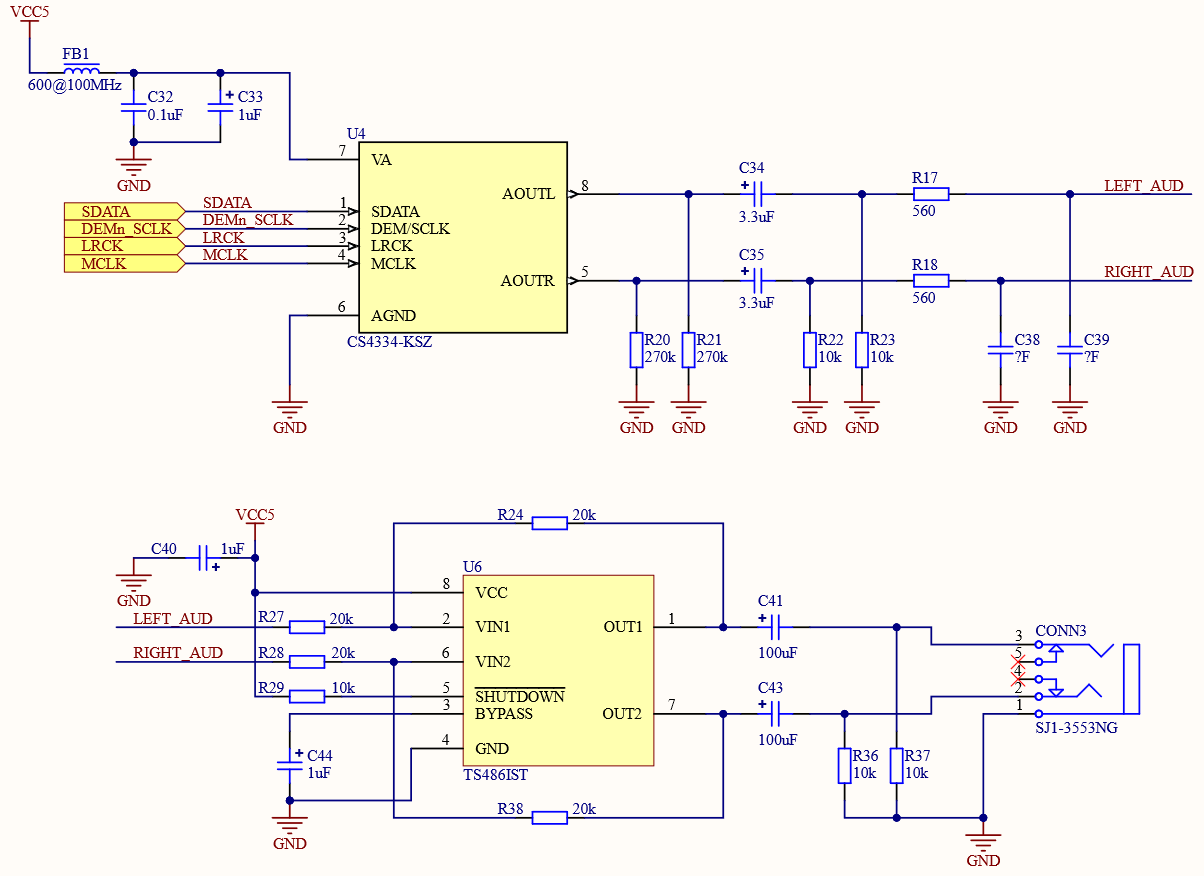
\includegraphics[width=150mm, keepaspectratio]{figures/DAC-AMP-JACK}
		\caption{NES audió jelért felelős áramkörök}
		\label{fig:DAC-AMP-JACK}
	\end{figure}
	
	Az erősítő komponensnek egy fázis fordító erősítőt választottam, amely erősítése az R24 és R38 ellenállásokkal módosítható a következő képletek alapján:
	
	\begin{align}	
		Gain_{LINEAR} = -\frac{RFEED}{RIN}
	\end{align} 
	
	\begin{align}	
		Gain_{dB} = 20 * lg(\frac{RFEED}{RIN})
	\end{align}
 
	Az áramkörben jelenleg nem állítottam be erősítést az RFEED és RIN ellenállások értékét 20 k$\Omega$-nak határoztam meg. Ez természetesen a hardveres tesztelés során cserélhető és állítható.	
	
\section{HDMI és I2C szint illesztő}
	\label{sec:HMI-I2C}
	
	A NES nyomtatott huzalozott kártyáján elhelyeztem egy HDMI csatlakozót és a körülötte elhelyezkedő áramkör segítségével felkészítettem VGA jelek kiadására. A teljes áramkör sematikus ábráját (schematic) \aref{sec:HDMI-MicroSDcard} függelékben láthatjuk.
	
	A jövőbeli fejlesztések miatt elhelyeztem a nyákon még egy I2C jel szint illesztőt is, amely segítségével az FPGA 3.3 V-on működő lábait, a HDMI audió jel kiadásáért felelős lábaihoz (SCL/SDA) illesztem. Így a kártya támogatja a TV-k és monitorok beépített hangszóróit is. 
	
	Az alábbi ábrákon láthatjuk és olvashatjuk egy HDMI anya aljzat pin és láb kiosztását:   
	
	\begin{figure}[H]
	\begin{minipage}[]{\textwidth}
		\begin{minipage}[b]{0.39\textwidth}
			\centering
			\includegraphics[width=55mm, keepaspectratio]{figures/hdmi-Pinout}
			\captionof{figure}{aljzat anya}
			\label{fig:HDMI-pinout}
		\end{minipage}
		\hfill
		\begin{minipage}[b]{0.59\textwidth}
			\footnotesize
			\centering
			\begin{tabular}{|l|c|l|c|}
				\hline
				\rowcolor[HTML]{C0C0C0} 
				\textbf{Funkció}  & \multicolumn{1}{l|}{\cellcolor[HTML]{C0C0C0}{\color[HTML]{333333} \textbf{Láb}}} & \textbf{Funkció}  & \multicolumn{1}{l|}{\cellcolor[HTML]{C0C0C0}{\color[HTML]{333333} \textbf{Láb}}} \\ \hline
				TMDS Data2+       & 1                                                                                & TMDS Clock Shield & 11                                                                               \\ \hline
				TMDS Data2 Shield & 2                                                                                & TMDS Clock-       & 12                                                                               \\ \hline
				TMDS Data-        & 3                                                                                & CEC               & 13                                                                               \\ \hline
				TMDS Data1+       & 4                                                                                & Reserved          & 14                                                                               \\ \hline
				TMDS Data1 Shield & 5                                                                                & SCL               & 15                                                                               \\ \hline
				TMDS Data1-       & 6                                                                                & SDA               & 16                                                                               \\ \hline
				TMDS Data0+       & 7                                                                                & DDC/CEC Ground    & 17                                                                               \\ \hline
				TMDS Data0 Shield & 8                                                                                & +5 V Power        & 18                                                                               \\ \hline
				TMDS Data0-       & 9                                                                                & Hot Plug Detected & 19                                                                               \\ \hline
				TMDS Clock+       & 10                                                                               &                   & \multicolumn{1}{l|}{}                                                            \\ \hline
			\end{tabular}
			\captionof{table}{HDMI lábkiosztás}
			\label{tab:HDMI-pinout}
		\end{minipage}
	\end{minipage}
	\end{figure} 
	
	Mivel az FPGA nem minden I/O láb pára képes differenciális jelek küldésére, ezért figyelni kell, hogy a csatlakozót az FPGA melyik oldalához közel helyezem el. A HDMI szabvány az adat vonalak között 100 $\Omega$-os impedancia különbséget ír elő (15\% os toleranciával), ezért érdemes ezeket az vezetékeket minél rövidebben/egyszerűbben megoldani (FPGA bekötési oldalhoz közel). 
	
	Az alkatrészeim védelmére a HDMI 5 V-os tápellátását egy 100 mA-es biztosítékon (poli fuse) vezettem keresztül, ez túláram esetén véd. A csatlakozó fém burkolatát egy 1 M$\Omega$-os ellenállással és egy 1 nF-os (1 kV-os) kapacitással földeltem, ez HDMI kimenetek esetén ideális. 
	
\section{A kártya bemenetei}
	
	A NES nyomtatott huzalozott kártyáját az eredeti játékkonzol kontroller csatlakozóival láttam el. Az eredeti kontroller a NES 5 V-járól működik, viszont a benne található parallel-soros átalakító (shift regiszter) adatlapja alapján 3.3 V-ról is működik. Ez azért fontos, mert így nem kell extra jelszint illesztő IC a kártyára, működtethetem az adat fogadást és az órajel küldést az FPGA I/O lábairól (3.3 V).
	
	Ennek a kontrollernek egyedi hét lábas anya csatlakozója, van amit \aref{fig:7PIN-Port} ábrán láthatunk.   
	
	\begin{figure}[H]
		\centering
		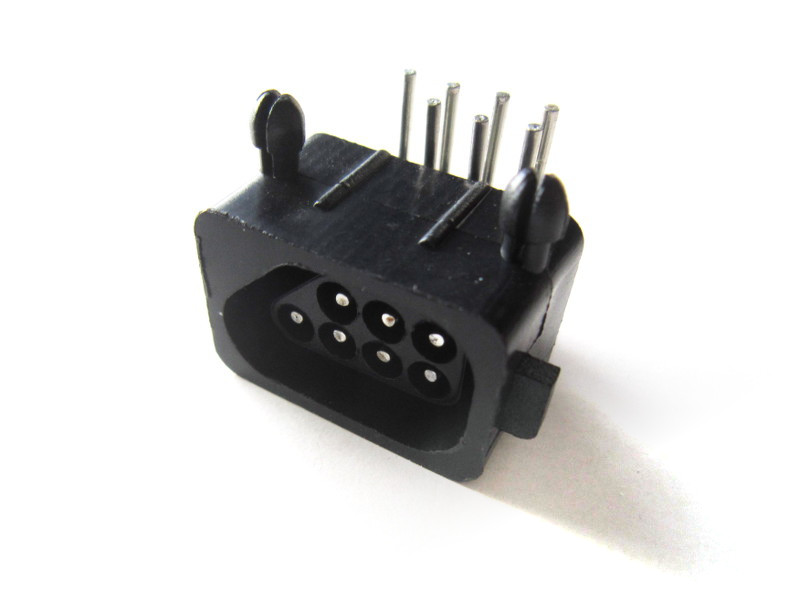
\includegraphics[width=80mm, keepaspectratio]{figures/7pin-connector} %110
		\caption{NES kontroller csatlakozó}
		\label{fig:7PIN-Port}
	\end{figure}
	
	Ebből a hét lábból kettőnek csak rögzítési szerepe van, kettő a tápellátásért felelős és a maradék három lábon keresztül történik a kontrollerben található regiszter olvasása, vezérlése és a működési órajel küldése. A kártyára ebből a csatlakozóból kettőt helyeztem el a kooperatív játékok végett. A kontroller portok sematikus ábráját (schematic) \aref{sec:DAC-controllers} függelékben láthatjuk.
	
	A pcb-n két gomb is helyet kapott az egyik az FPGA és ezáltal a NES reset gombja (RST), a másik pedig az FPGA újrakonfigurálását elindító nyomógomb (PROG). Az RST gomb pergésmentesítésért az FPGA a felelős. Ezek mindegyikét \aref{sec:OSC-JTAG} függelékben láthatjuk. 
	
\section{MicroSD kártya}
	
	A MicroSD kártya csatlakozót teljes interfésszel tudtam implementálni, mivel az FPGA-nak még sok szabad I/O lába maradt. Ez azt jelenti hogy teljes SD kártya protokollt is megtudok valósítani a NES fejlesztő kártyán, az egyszerűbb soros SPI kommunikációt mellett/helyett. A MicroSD kártya segéd áramkörét \aref{sec:HDMI-MicroSDcard} függelék sematikus rajzán láthatjuk. 
	
	Itt érdemes az áramkör ki-bekapcsolásáért felelős P-Mosfet-es áramkört megnézni, ez azért szükséges, mert a fent említett két protokoll közötti váltáshoz áramtalanítanunk kell az csatlakozót. A tápellátás elvétele mellet a felhúzó ellenállások tápellátását is elvesszük kikapcsolás során. Egyedül a CD kártya detektáló lábtól nem vesszük el, mivel ez csak azt jelzi, hogy van-e SD kártya a csatlakozóban (nem része a fent említett kommunikációs protokolloknak). Ezt be/ki kapcsolási eseményt az FPGA egy I/O lábának segítségével kontrollálhatjuk.
	
	Az FPGA védelme érdekében elhelyeztem a az SD kártya CLK lábára egy 33 $\Omega$-os soros ellenállást, ezt a PCB layout tervezése során a lehető legközelebb helyeztem el az FPGA-hoz.  
	
\section{FPGA konfigurációs módok}
	
	A NES kártyának is, a LOGSYS Spartan-6 FPGA kártyához hasonló módon \cite{spatan6} két konfigurációs módja van. Az FPGA-t felprogramozhatjuk a fejlesztőportban található JTAG interfész segítségével, illetve felkonfigurálhatja saját magát a kártyán található soros FLASH memóriából is. A konfigurációs módok között egy rövidzár segítségével (jumper) válthatunk a LOGSYS-es kártyához hasonlóan. Ennek működését \aref{tab:FPGA-config} táblázatban olvashatjuk, illetve \aref{sec:FPGA-BANKS} függelékben láthatjuk.       
	
	\begin{table}[H]
		\footnotesize
		\centering
		\begin{tabular}{|c|c|l|}
			\hline
			\rowcolor[HTML]{C0C0C0} 
			\textbf{\begin{tabular}[c]{@{}c@{}}Jumper\\ állása\end{tabular}} & {\color[HTML]{333333} \textbf{\begin{tabular}[c]{@{}c@{}}Konfigurációs \\ mód\end{tabular}}} & \multicolumn{1}{c|}{\cellcolor[HTML]{C0C0C0}\textbf{Leírás}}                                                                                                                          \\ \hline
			\rowcolor[HTML]{FFFFFF} 
			\raisebox{-.5\height}{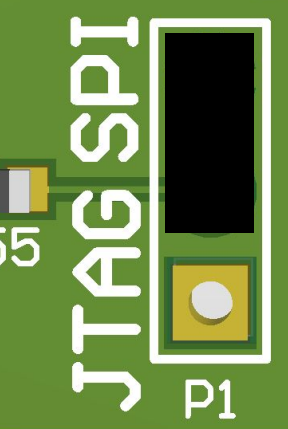
\includegraphics[width=10mm, keepaspectratio]{figures/SPI-jumper}}                                                                & JTAG                                                                                         & Az FPGA-t a JTAG interfacen keresztül kell felkonfigurálni.                                                                                                                           \\ \hline
			\rowcolor[HTML]{FFFFFF} 
			\raisebox{-.5\height}{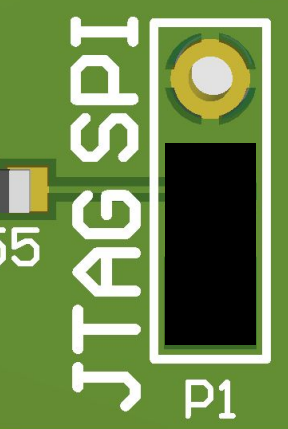
\includegraphics[width=10mm, keepaspectratio]{figures/JTAG-jumper}}                                                                & SPI                                                                                          & \begin{tabular}[c]{@{}l@{}}Az FPGA az SPI buszos soros FLASH memóriából konfigurálja \\ fel magát a tápfeszültség bekapcsolása vagy a PROG gomb \\ megnyomását követően.\end{tabular} \\ \hline
		\end{tabular}
		\caption{Fejlesztői port bekötése}
		\label{tab:FPGA-config}
	\end{table}
	
\section{Soros Flash memória}
	
	A NES kártyán egy Atmel AT25DF321A típusú, 32 Megabit-es SPI busszal rendelkező soros FLASH memóriát helyeztem el. Ez a komponens az FPGA számára konfigurációs memóriaként szolgál (tehát a NES hardverének binárisát fogja tartalmazni). Ennek a komponensnek az elhelyezése, bekötése és ezáltal működése is megegyezik a Logsys Spartan-6-os fejlesztői kártyán található Flash-el \cite{spatan6}. A soros Flash bekötését, pedig \aref{sec:SRAM-SPI-Flash} függelékben láthatjuk.
	
	%TODO fix jumper heights if you have time
\section{LOGSYS fejlesztői port}
	
	A fejlesztői port kialakítása teljes mértékben megegyezik a Logsys fejlesztő kártyán található port-al, ennek köszönhetően az FPGA felprogramozása történhet a MIT tanszéken tervezett egyedi fejlesztő kábellel. Ennek részletes bemutatása \acite{spatan6}-os dokumentáció része. A fejlesztői port kialakítását \aref{fig:DEV-port} képen látható és FPGA bekötését pedig \aref{tab:DEV-pinout} táblázatban olvasható, illetve \aref{sec:OSC-JTAG} függelékben látható. Az FPGA sikeres felkonfigurálását egy zöld LED-el jelzem (DONE). %A fejlesztői port a következő elemekből áll:
	
%	\begin{enumerate}
%		\item JTAG interfész (vörös)
%		\item Soros SPI kommunikációs interfész (zöld)
%		\item 5 V-os egyenfeszültségű táp forrás (szürke)
%	\end{enumerate}
%	
%	\begin{figure}[H]
%		\begin{minipage}[]{\textwidth}
%			\begin{minipage}[b]{0.49\textwidth}
%				\centering
%				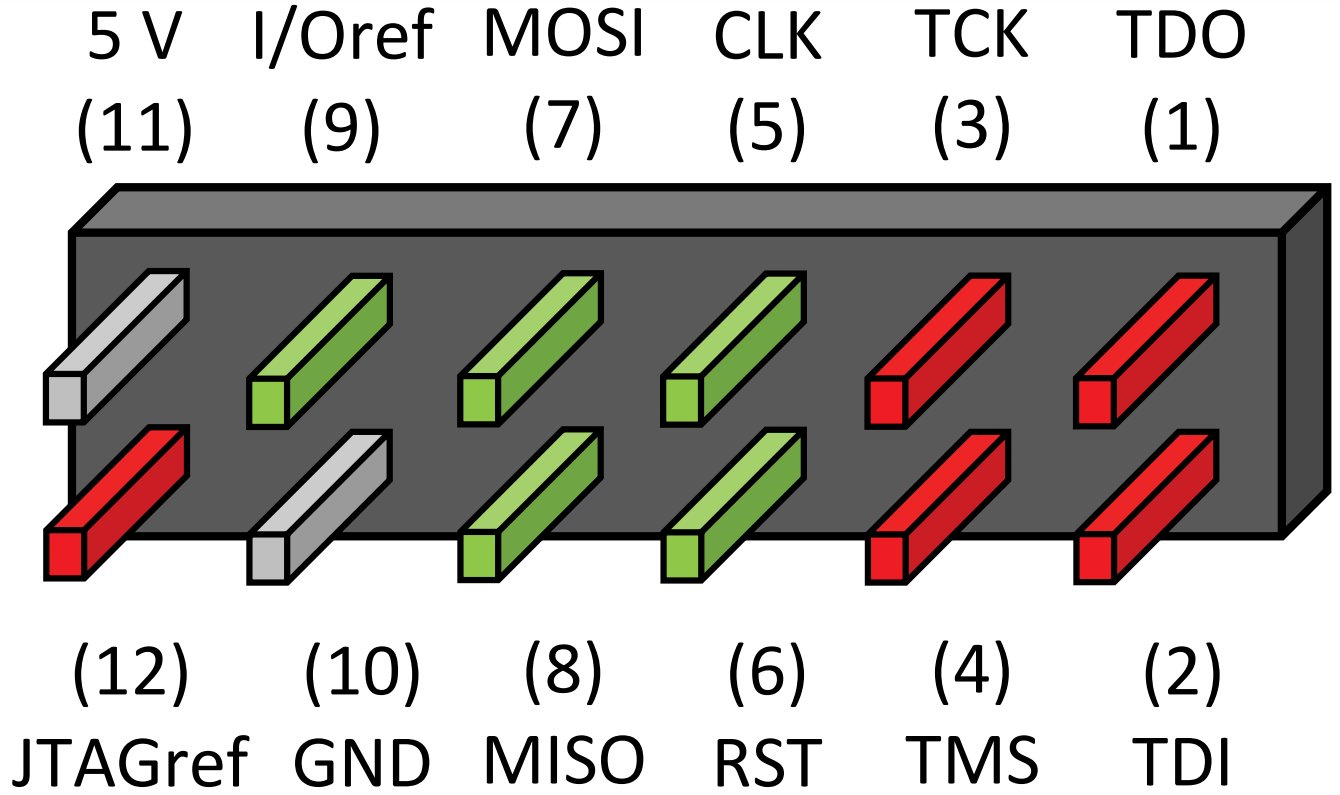
\includegraphics[width=50mm, keepaspectratio]{figures/DEV-port}
%				\captionof{figure}{Fejlesztői port kiosztása}
%				\label{fig:DEV-port}
%			\end{minipage}
%			\hfill
%			\begin{minipage}[b]{0.49\textwidth}
%				\footnotesize
%				\centering
%				\begin{tabular}{|l|l|l}
%					\cline{1-2}
%					\rowcolor[HTML]{C0C0C0} 
%					\multicolumn{1}{|c|}{\cellcolor[HTML]{C0C0C0}\textbf{jel}} & \multicolumn{1}{c|}{\cellcolor[HTML]{C0C0C0}{\color[HTML]{333333} \textbf{Irány}}} & \multicolumn{1}{c}{\cellcolor[HTML]{C0C0C0}\textbf{FPGA láb}} \\ \hline
%					\rowcolor[HTML]{FFFFFF} 
%					MOSI                                                       & bemenet                                                                            & \multicolumn{1}{l|}{\cellcolor[HTML]{FFFFFF}P104}             \\ \hline
%					\rowcolor[HTML]{FFFFFF} 
%					MISO                                                       & kimenet                                                                            & \multicolumn{1}{l|}{\cellcolor[HTML]{FFFFFF}P144}             \\ \hline
%					CLK                                                        & bemenet                                                                            & \multicolumn{1}{l|}{P95}                                      \\ \hline
%					RST                                                        & bemenet                                                                            & \multicolumn{1}{l|}{P94}                                      \\ \hline
%				\end{tabular}
%				\captionof{table}{Fejlesztői port bekötése}
%				\label{tab:DEV-pinout}
%			\end{minipage}
%		\end{minipage}
%	\end{figure} 		

\section{Nyomtatott áramköri terv}

A schematik megalkotását követően, a pcb tervezés következő fázisa a layout (pcb rajzolat) elkészítése. Itt természetesen figyelembe kell vennünk az eddig meghatározott célokat \ref{sec:Size}, miszerint egy kompakt hordozható eszközt tervezünk. Egy nyomtatott áramkör mérete nagyban függ a réteg felépítésétől, illetve a kiválasztott komponensek méretétől. Tehát minél több rétegből épül fel egy pcb és minél modernebb alkatrészeket használunk, annál nagyobb felületi alkatrész sűrűség érhető el. Természetesen ezekkel arányosán az ár is nő. Viszont mivel először egy prototípust fejlesztek, ezért egy kompromisszumos megoldást kellett választanom.   
		
	\subsection{Réteg beállítások}
	
	A Logsys Spartan-6-os fejlesztő kártyán már láthattuk \cite{spatan6}, hogy a választott FPGA chip TQFP tokozása miatt, két rétegű nyákon behuzalozható. Az FPGA NES kártya tervezésekor ez egy fő szempont volt, mivel így érdekes mérnöki megoldásokat kellett alkalmaznom a táp bekötése során, illetve a kártya elkészítési költségét is csökkenteni tudtam.
	
	A prototípus kártyákat a jlcpcb nevű kínai nyomtatott áramkör gyártó fogja gyártani. Ahhoz, hogy az Altium tervező program képes legyen bonyolultabb számítások (differencial pair routing) és szimulációk készítésére, a réteg felépítést meg kell adnunk a PCB-nk számára. Ez a kínai gyártó által szolgáltatott információk által \cite{jlcpcb} alakítottam ki, ez \aref{fig:Layer-stackup} ábrán látható.    
	
	\begin{figure}[H]
		\centering
		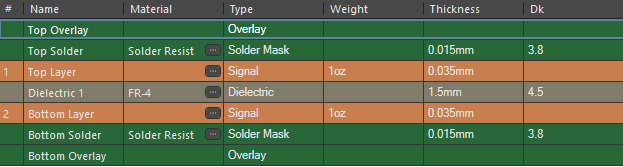
\includegraphics[width=150mm, keepaspectratio]{figures/Layer-stackup}
		\caption{Az FPGA NES kártya réteg beállításai}
		\label{fig:Layer-stackup}
	\end{figure}
	
	\subsection{Komponensek elhelyezése}
	
	A rétegbeállításokat követően, a komponensek és segéd áramköreik elhelyezése következett. Ennek segítségével tudtam meghatározni végül, hogy az FPGA mely I/O bankjaihoz/lábaihoz fogom vezetni a különböző komponensek kivezetéseit, illetve ez határozta meg pcb-m méreteit is. Az alkatrészek és segéd áramköreik rajzolatát \aref{sec:NES-components} függelékben láthatjuk, de a könnyebb áttekinthetőség érdekeben elkészítettem a következő ábrát:
	
	\begin{figure}[H]
		\centering
		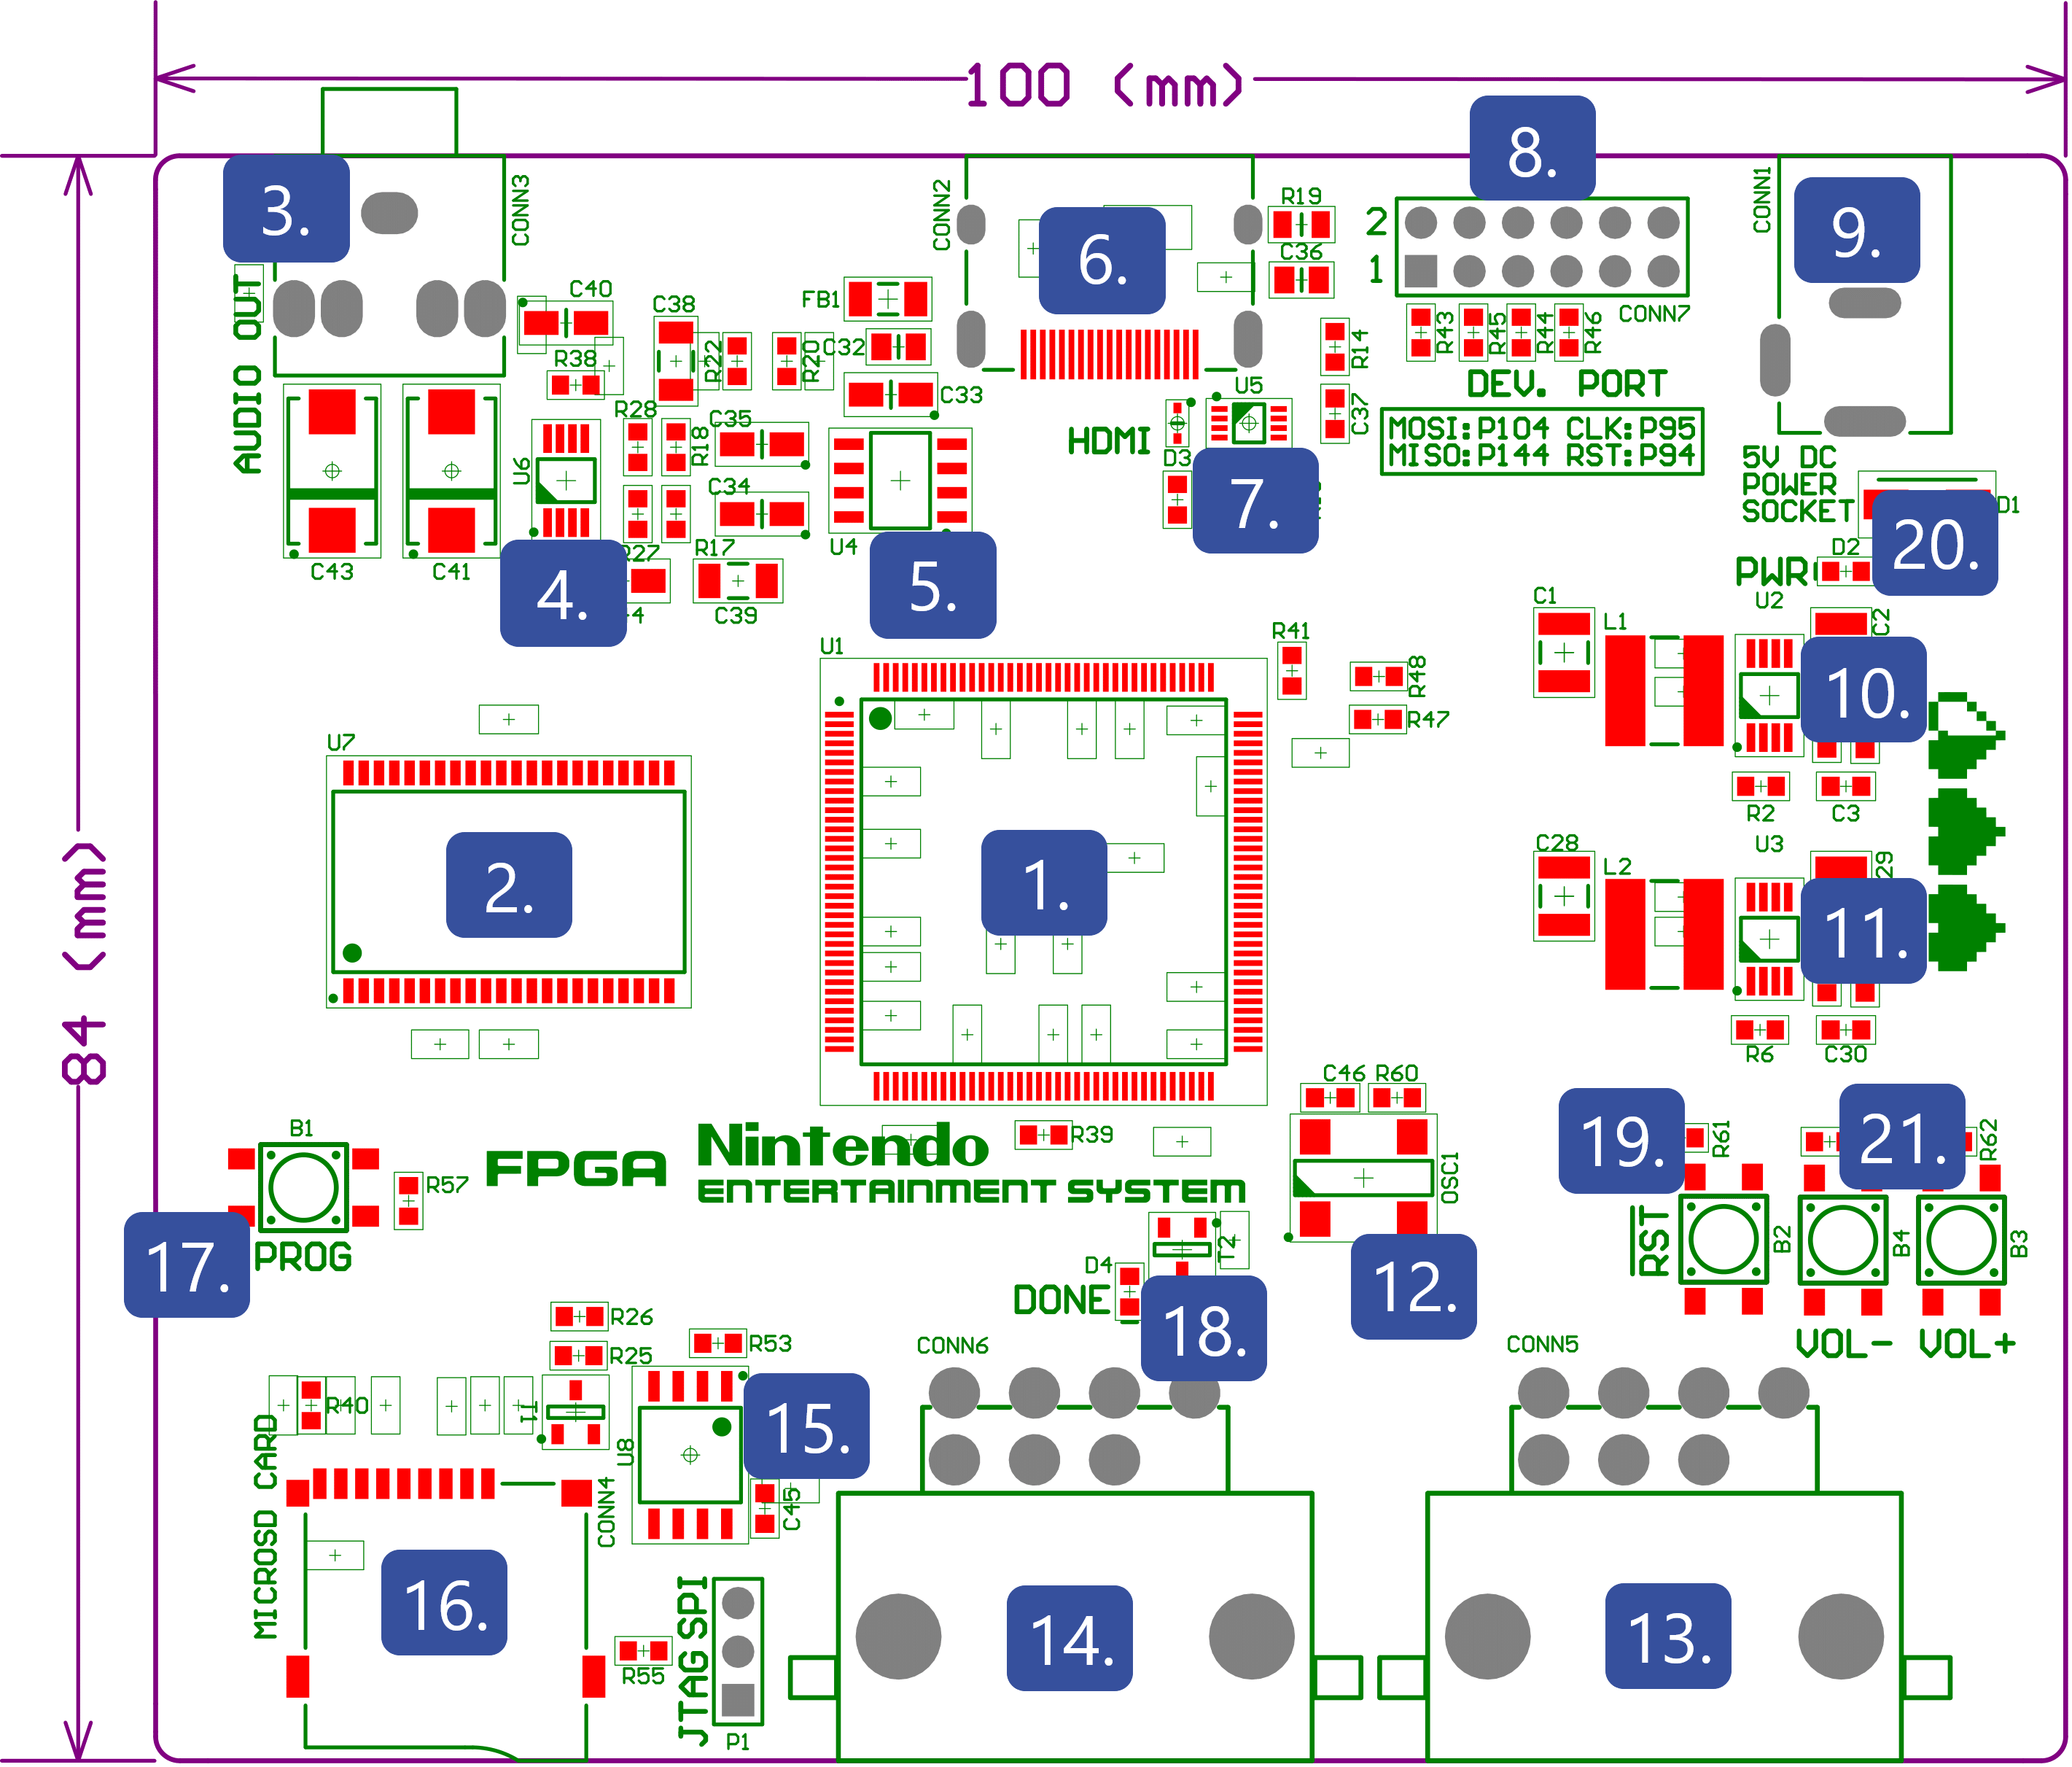
\includegraphics[width=135mm, keepaspectratio]{figures/components-top}
		\caption{A top layer alkatrész elhelyezési terve} 
		\label{fig:NES-components-top}
	\end{figure}
	
	FPGA NES kártya főbb alkotó komponensei:
	\begin{enumerate}
		\item Xilinx XC6SLX9-2TQG144C típusú FPGA
		\item 256k x 16 bites (512 kB), 10 ns-os aszinkron SRAM (Cypress CY7C1041DV33-10ZSXI)
		\item 3.5mm Jack csatlakozó (CUI SJ1-3553NG)
		\item 100mW Erősítő (TS486IST fülhallgatókhoz)
		\item Digital Analog Converter (DAC), (CS4334-KSZ)
		\item HDMI csatlakozó
		\item 2C szint illesztő (PCA9306DCUR)
		\item Csatlakozó a LOGSYS fejlesztői kábel számára
		\item 2.1mm 12 V / 5 A DC táp csatlakozó (DC10A)
		\item 3,3 V feszültséget előállító tápegység
		\item 1,2 V feszültséget előállító tápegység
		\item 50 MHz-es oszcillátor 
		\item 7 pines NES GamePAD kontroller csatlakozók anya aljzat 1
		\item 7 pines NES GamePAD kontroller csatlakozók anya aljzat 2
		\item 32 Mbites SPI buszos soros FLASH (Atmel AT25DF321A)
		\item MicroSD kártya foglalat
		\item Az FPGA újrakonfigurálását indító gomb (PROG)
		\item Az FPGA sikeres felkonfigurálását jelző LED (DONE)
		\item Az FPGA kézi reset gomja (RSTn)
		\item A bekapcsolt tápfeszültséget jelző LED (PWR)
		\item A NES hangerő szabályzó gombjai (VOL-, VOL+)
	\end{enumerate}
	
	Mivel kézi forrasztással és hőfúvó segítségével fogjuk a kártyát összeállítani, ezért törekedtem arra, hogy az összes komponens (és ezek segéd áramkörei) a előlapi (top) oldalon helyezkedjen el, illetve a hátoldalra (bottom) csak azonos méretű elemek kerüljenek. Egyedül a HDMI csatlakozó biztosítéka került a hátoldalra, ami nem 0603-as méretű lett.
	
	Ezt követően a PCB alkatrészek bekötésével foglalkoztam, itt a alsó és felső réteget is jel/föld (signal/GND) rétegként alakítottam ki. Ez azt jelenti, hogy jel vezetékeket és táp vonalak bekötését követően az egész nyák felszínén föld kitöltést hoztam létre, így növelve a jelek integritását. A alsó és a felső föld rétegeket, pedig via-k segítségével kötöttem össze (via stiching). A két rétegemet egyszerre \aref{sec:FPGA-nes-transparency} függelékben láthatjuk, az itt használt réteg ábrázolási mód az Altium designer átlátszó 2D módja, amely betekintést enged a föld kitöltések alá. A felső réteg jeleit és komponensek pad-jei vörös színnel vannak jelölve, a alsó rétegé pedig kék színnel.
	
	\subsection{HDMI adatvonalainak bekötése}
	
	A HDMI vonalak kialakításáról már \aref{sec:HMI-I2C} fejezet során olvashattunk. Viszont mivel a réteg kialakítás során a két rétegű megvalósítást választottunk és a PCB gyártó (jlcpcb) nem biztosít két réteg esetén impedancia kontrollálásra réteg felépítést. Ezért a HDMI szabványban leírt 100 $\Omega$-os impedancia különbséget (15\% os toleranciával) csak egy speciális differenciális pár bekötés típussal tudjuk biztosítani. Ez a típus a Dual Strip Coplanar Waweguide Grounded, ez azt jelenti, hogy differenciális pár bekötés mellett figyelnünk kell arra is, hogy a pár jobb és bal oldalán fix távolságra föld kitöltést helyezzünk el. Az itt található két réteg földjét előre meghatározott távolságokon via fence-szel látjuk el (ezt az elrendezést \aref{fig:coplanar} ábrán láthatjuk). A via-k közti maximális távolságot a következő képlettel számolhatjuk ki:
	
	\begin{align}
		\label{mat:via-distance}	
		S(via) = \frac{\lambda}{20} = \frac{c}{20 * f * \sqrt[]{\epsilon_r}}
	\end{align}   
	
	Az \ref{mat:via-distance} képletben található $\lambda$ a differenciális jelünk hullámhossza (a részletesebb képletben pedig: c a fény terjedési sebessége, f a jelünk frekvenciája, $\epsilon_r$ pedig az anyag dielektromos állandója). A mi esetünkben ezen a vezeték páron 250 Mhz-es jeleket fogunk küldeni, ennek hullámhossza körülbelül 1,151 m, ebből kiszámított két via közti maximális távolság 0.058 m (ennél természetesen választhatunk kisebb értéket is).
	
	\begin{figure}[H]
		\centering
		\includegraphics[width=90mm, keepaspectratio]{figures/coplanar}
		\caption{Dual Strip Coplanar Waweguide Grounded felépítése} 
		\label{fig:coplanar}
	\end{figure}
	
	Az Altium designer segítségével van lehetőségem a GND réteg és vezető pár közti távolság kiszámítására (később az ecad szoftver ez alapján fogja elhelyezni a vezetékeket). Ezek a beállítások az alábbi ábrán láthatók:      
	
	\begin{figure}[H]
		\centering
		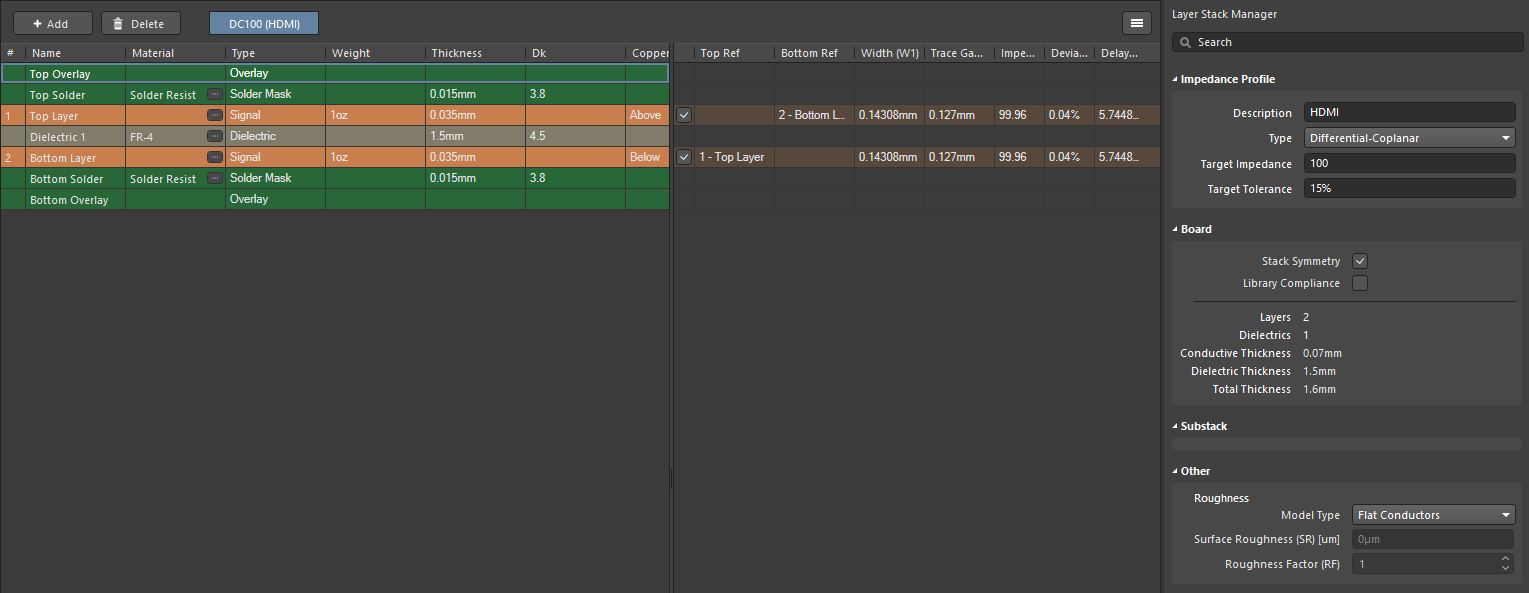
\includegraphics[width=150mm, keepaspectratio]{figures/Impedance-control}
		\caption{Coplanar differential pair routings Altium beállításai}
		\label{fig:Impedance-control}
	\end{figure}
	
	A FPGA NES kártya HDMI jeleinek bekötésére 2,75 mm-es via fence méretet választottam (körülbelül a fentebb kiszámolt érték 20-ad része) ez részletesen \aref{fig:HDMI-Differencial-pair-routing} ábrán látható, amely \aref{sec:FPGA-nes-transparency} függelékből lett kiemelve.
	
	\begin{figure}[H]
	\centering
	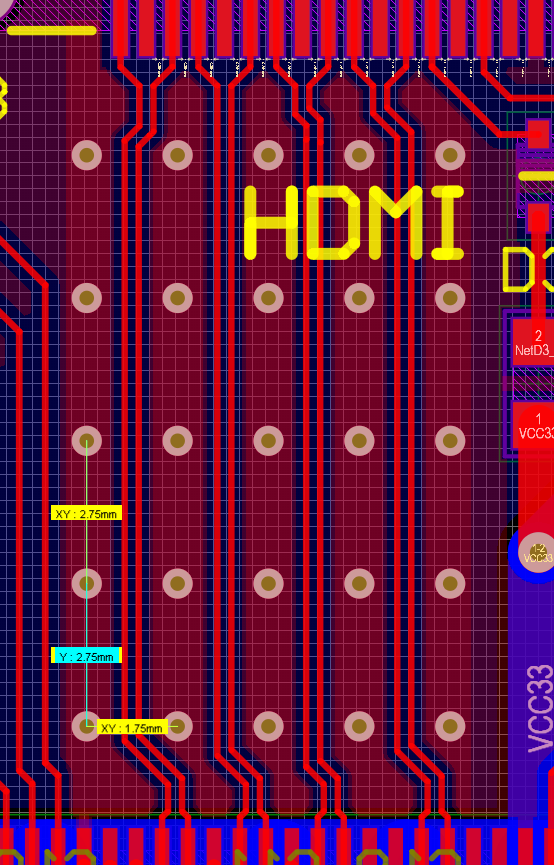
\includegraphics[width=82mm, keepaspectratio, angle=90]{figures/HDMI-Differencial-pair-routing}
	\caption{A HDMI adatvonalainak bekötése}
	\label{fig:HDMI-Differencial-pair-routing}
	\end{figure}
	
	\subsection{FPGA táp vonalak kialakítása}
	
	Ahhoz, hogy a Spartan-6-os FPGA chip-et két rétegen teljes mértékben ki tudjuk használni egy speciális tápellátási módszerhez kellet folyamodnunk (Logsys-es fejlesztő kártya táp vonalai is hasonlóan vannak kialakítva). Ennek alapja az volt, hogy az alsó oldalról érkezik a 3.3 V és az 1.2 V-is. A 3.3 V-ot az FPGA lábai alatt végig vezetjük (innen indul ki a többi 3.3 V-os komponens tápellátást is) egy helyen be engedve az 1.2 V-ot a belső magja számára. Ezzel a rendszerrel az előnye, hogy így az összes csatoló (coupling) és hidegítő (bulk) kapacitás az FPGA alatt kaphat helyet, ezzel szabadon tartva a top réteget az FPGA I/O bankjainak és JTAG interfészének bekötésére.
	
	\begin{figure}[H]
		\centering
		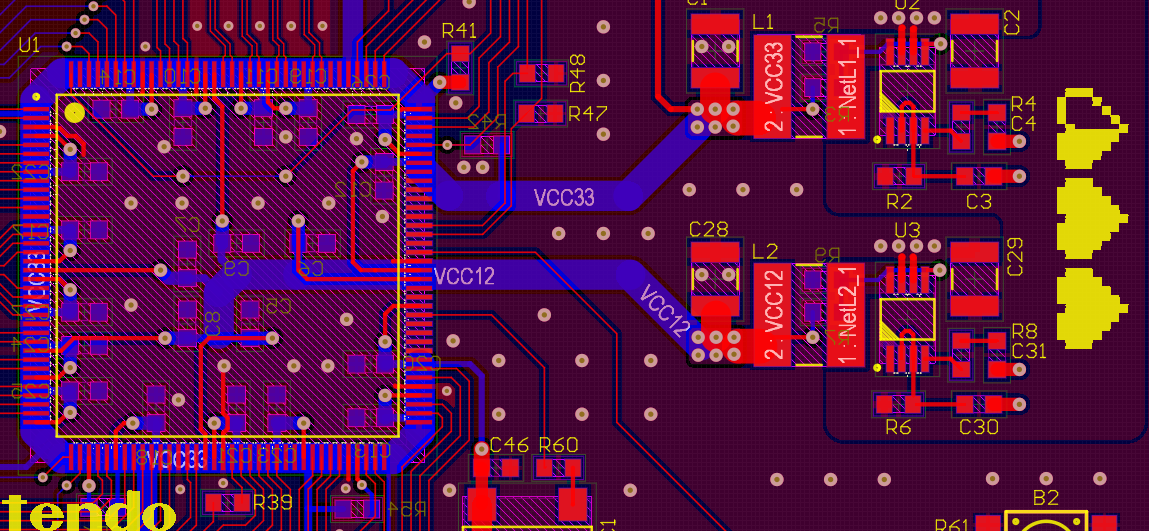
\includegraphics[width=150mm, keepaspectratio]{figures/FPGA-PSU-routing}
		\caption{FPGA tápellátásának kialakítása}
		\label{fig:FPGA-PSU-routing}
	\end{figure}
	
	A chip tápellátását \aref{fig:FPGA-PSU-routing} ábrán láthatjuk, a kártya teljes tápellátását pedig \aref{sec:FPGA-nes-transparency} függelékben figyelhetjük meg. 
	
	\subsection{FPGA NES 3D terve}
	
	A kártya tervezését követően, az Altium designer lehetőséget nyújt PCB 3D tervének megtekintéséhez (ez a komponensek elhelyezésénél, illetve nyák foglalatok/tokok tervezésénél is hasznos). Ez egy teljes képet nyújt a nyomtatott áramkör kialakításáról és jövőbeli kinézetéről. Az FPGA NES 3D tervét a következő (\ref{fig:PCB-3D}) ábrán láthatjuk:  
	
	\begin{figure}[H]
		\centering
		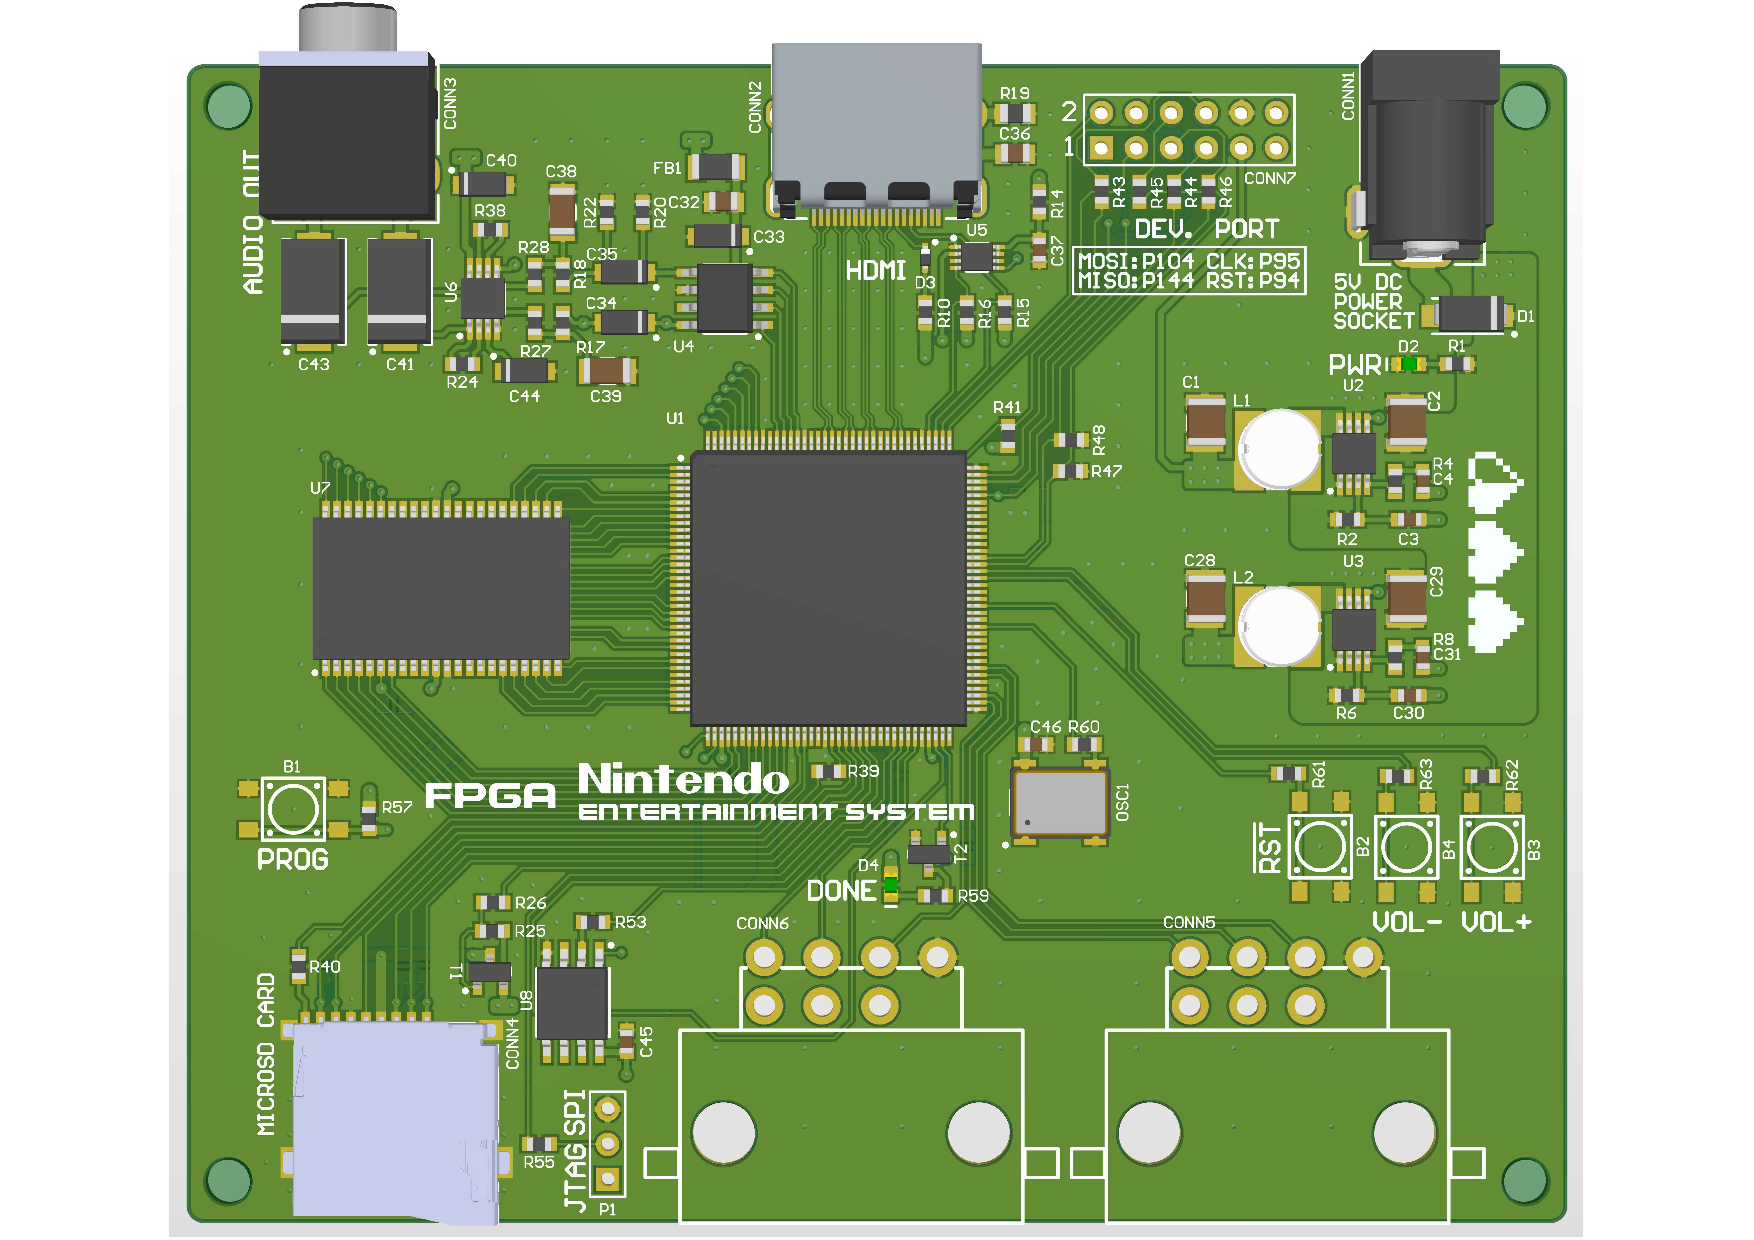
\includegraphics[width=100mm, keepaspectratio, angle=90]{figures/Top}
		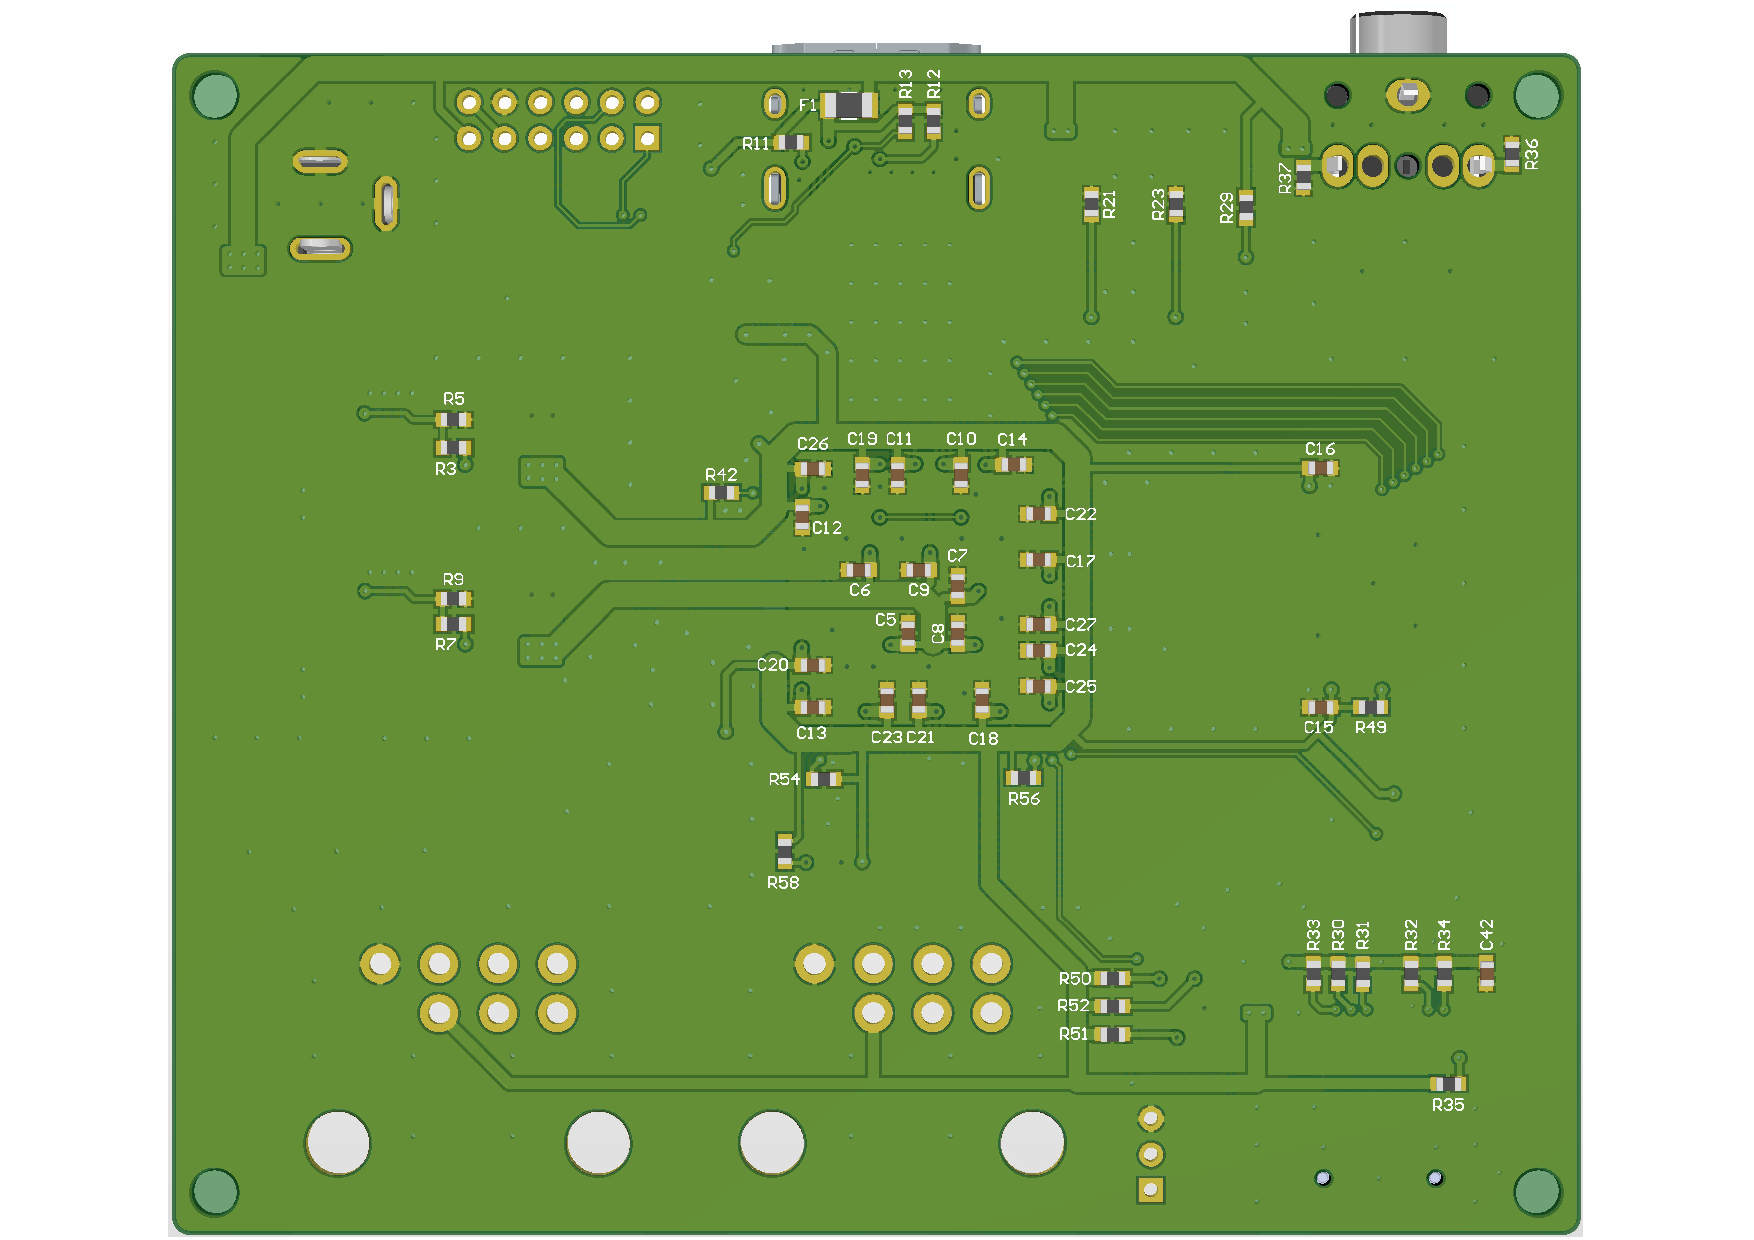
\includegraphics[width=100mm, keepaspectratio, angle=90]{figures/Bottom}
		\caption{3D PCB rajzolat} 
		\label{fig:PCB-3D}
	\end{figure}
	

	
	
	
	

